\documentclass[sigconf]{acmart}
\pdfmapfile{+libertine.map}
\pdfmapfile{+newtx.map}
\pdfmapfile{+zi4.map}

%% Submission to BID 2026 (ICPP '26 workshop) -- single blind, max 8 pages incl. references
\setcopyright{none}
\settopmatter{printacmref=false}
\renewcommand\footnotetextcopyrightpermission[1]{}
\pagestyle{plain}
\acmConference[BID '26]{Benchmarking in the Data Center: Workshop at ICPP 2026}{September 28, 2026}{Singapore}
\acmBooktitle{Benchmarking in the Data Center (BID '26), Workshop at the 55th International Conference on Parallel Processing (ICPP 2026), September 28, 2026, Singapore}

\usepackage{booktabs}

\begin{document}

\title[When One Node Beats Two]{When One Node Beats Two: Benchmarking DeepSeek-R1 Inference with SGLang on H100 and H200 Systems}

\author{Luca Lowndes}
\affiliation{%
  \institution{Monash DeepNeuron, Monash University}
  \city{Melbourne}
  \country{Australia}}
\email{luca.lowndes@example.com}

\author{Nathan SURNAME}
\affiliation{%
  \institution{Monash DeepNeuron, Monash University}
  \city{Melbourne}
  \country{Australia}}
\email{nathan@example.com}

\begin{abstract}
Serving trillion-scale mixture-of-experts (MoE) language models is rapidly becoming a first-class high-performance computing workload, yet published guidance on configuring inference frameworks for real clusters remains scarce. We present a systematic benchmarking study of offline inference throughput for DeepSeek-R1 (671B parameters, 37B active) served with SGLang, carried out on two production GPU systems: the NSCC Singapore ASPIRE-2A+ supercomputer (8$\times$H100 nodes) and an H200-based AI cluster. Under a fixed benchmark protocol---2{,}000 ShareGPT prompts, offline batch inference, a 420-second wall-clock budget---we evaluate the software stack (CUDA version, containerization), scaling architecture (one node versus two), scheduler memory policy, hybrid tensor/data/pipeline parallelism, and more than 40 manual NCCL network configurations.

Three findings stand out. First, configuration dominates hardware quantity: a tuned single node (8$\times$H200) reaches 17{,}417 tok/s, an 81\% improvement over the untuned two-node, 16-GPU baseline (9{,}611 tok/s), and it also outperforms the best two-node configuration we found (17{,}032 tok/s) while using half the GPUs---a 2.05$\times$ per-GPU efficiency advantage. The best configuration combines pipeline parallelism across NUMA-local GPU groups (PP=2), tensor parallelism inside each group (TP=4), and SGLang's data-parallel attention (DP=4), which eliminates redundant multi-head-latent-attention KV-cache replication. Second, the highest-leverage optimizations are unglamorous: aligning the CUDA toolkit version (+35\%), running inside a Singularity container (+12\%), and saturating the KV-cache with large batches. Third, exhaustive manual NCCL tuning is a well-characterized dead end: none of our 40+ hand-tuned configurations matched NCCL's autotuned defaults, a null result that cleanly attributes the multi-node penalty to fundamental inter-node latency rather than misconfiguration. We distill these results into practical guidance for provisioning LLM inference on HPC and data-center GPU systems.
\end{abstract}

\begin{CCSXML}
<ccs2012>
 <concept>
  <concept_id>10011007.10010940.10010992.10010998</concept_id>
  <concept_desc>Software and its engineering~Software performance</concept_desc>
  <concept_significance>500</concept_significance>
 </concept>
 <concept>
  <concept_id>10010520.10010521.10010528</concept_id>
  <concept_desc>Computer systems organization~Parallel architectures</concept_desc>
  <concept_significance>300</concept_significance>
 </concept>
 <concept>
  <concept_id>10002944.10011122.10002945</concept_id>
  <concept_desc>General and reference~Performance</concept_desc>
  <concept_significance>500</concept_significance>
 </concept>
</ccs2012>
\end{CCSXML}

\ccsdesc[500]{Software and its engineering~Software performance}
\ccsdesc[300]{Computer systems organization~Parallel architectures}
\ccsdesc[500]{General and reference~Performance}

\keywords{LLM inference, benchmarking, SGLang, DeepSeek-R1, tensor parallelism, pipeline parallelism, data-parallel attention, NCCL, GPU clusters}

\maketitle

\section{Introduction}
Large language model (LLM) inference has become a dominant workload in commercial data centers and, increasingly, on national supercomputing facilities. Unlike training, whose distributed-systems trade-offs are well documented~\cite{shoeybi2019megatron,narayanan2021efficient}, high-throughput \emph{inference} of very large mixture-of-experts (MoE) models remains an exercise in folklore: serving frameworks expose dozens of interacting knobs---parallelism layout, scheduler memory policy, communication settings, container runtime, CUDA toolkit---and the published literature offers little systematic evidence about which of them matter on real clusters.

This paper reports such evidence. As part of the 2025 APAC HPC-AI Competition~\cite{apachpcai2025}, we benchmarked offline inference throughput of DeepSeek-R1~\cite{deepseekr1}---a 671B-parameter MoE reasoning model with 37B active parameters per token---served with SGLang~\cite{zheng2024sglang} under a fixed, externally specified protocol: 2{,}000 ShareGPT prompts~\cite{sharegpt}, offline batch execution, fixed seed, and a hard 420-second budget that includes model instantiation and warm-up. The protocol makes total token throughput (tok/s) the single figure of merit, turning the exercise into a clean, reproducible benchmarking problem: given fixed hardware and a fixed workload, how far can software configuration alone move the number?

Quite far, it turns out. Across a measurement campaign on two production systems---the NSCC Singapore ASPIRE-2A+ supercomputer (nodes of 8$\times$NVIDIA H100) and an H200-based AI cluster---we improved throughput from a 9{,}611 tok/s two-node baseline to 17{,}417 tok/s \emph{on a single node}, an 81\% gain achieved while releasing half of the allocated GPUs. The best single-node configuration also outperforms the best two-node configuration we were able to construct (17{,}032 tok/s), doubling per-GPU efficiency (2{,}177 versus 1{,}065 tok/s per GPU).

Our contributions are:
\begin{itemize}
\item A log-verified, stepwise decomposition of a 1.81$\times$ throughput improvement into individual configuration decisions: CUDA toolkit alignment, containerization, scaling architecture, scheduler memory policy, and hybrid parallelism (Sections~\ref{sec:stack}--\ref{sec:hybrid}).
\item An empirical analysis of \emph{why} a hybrid TP4$\cdot$DP4$\cdot$PP2 layout with SGLang's data-parallel attention is the right shape for DeepSeek-R1 on an 8-GPU node: multi-head latent attention (MLA) has a single latent KV head, so pure tensor parallelism replicates the KV-cache on every rank; data-parallel attention removes that replication and returns the freed memory to the batch scheduler (Section~\ref{sec:hybrid}).
\item A deliberately reported null result: none of 40+ hand-tuned NCCL configurations (protocol, thread, channel, and RDMA settings) matches NCCL's autotuned defaults---evidence that the two-node penalty is fundamental to tightly coupled parallelism over the inter-node fabric, not a tuning artifact (Section~\ref{sec:nccl}).
\item Deployment guidance derived from the measurements: exhaust vertical scaling before horizontal; cross node boundaries with pipeline---not tensor---parallelism if you must; scale beyond a node by replicating tuned single-node workers behind a router (Section~\ref{sec:discussion}).
\end{itemize}

We release our build scripts, job scripts, and raw benchmark logs to support reproduction.

\section{Background}
\subsection{DeepSeek-R1 and MLA}
DeepSeek-R1~\cite{deepseekr1} shares the DeepSeek-V3 architecture~\cite{deepseekv3}: a decoder-only transformer in which most feed-forward blocks are MoE layers (256 routed experts plus one shared expert, 8 routed experts active per token), totalling 671B parameters of which roughly 37B are active per token. Its attention mechanism, multi-head latent attention (MLA), compresses keys and values into a single low-rank latent vector per token. MLA is central to this paper's results: because the compressed KV-cache has effectively \emph{one} KV head, tensor-parallel execution cannot shard it---each TP rank stores a full replica, multiplying KV-cache memory by the TP degree~\cite{sglangv04blog}. Since offline throughput is governed by how many requests fit in the KV-cache simultaneously (Section~\ref{sec:batch}), this replication directly taxes the achievable batch size.

\subsection{SGLang and its parallelism axes}
SGLang~\cite{zheng2024sglang} is an LLM serving framework built around RadixAttention prefix caching and a continuous batching scheduler in the lineage of Orca~\cite{yu2022orca} and vLLM~\cite{kwon2023vllm}. For multi-GPU execution it composes: \emph{tensor parallelism} (TP), which shards each weight matrix and requires an all-reduce per layer~\cite{shoeybi2019megatron}; \emph{pipeline parallelism} (PP), which assigns contiguous layer blocks to GPU groups and communicates only stage-boundary activations~\cite{huang2019gpipe}; \emph{expert parallelism} (EP), which distributes MoE experts; and \emph{data-parallel attention} (DP-attention), a DeepSeek-specific optimization in which attention is executed data-parallel across groups of ranks so each request's latent KV-cache lives on exactly one rank, eliminating the MLA replication described above~\cite{sglangv04blog}. SGLang requires the DP degree to divide the TP degree; enabling DP-attention also activates the framework's shared-expert optimizations. Two runtime knobs feature heavily in our study: \texttt{mem-fraction-static}, the fraction of GPU memory reserved for weights plus KV-cache, and \texttt{cuda-graph-max-bs}, the largest decode batch size for which CUDA graphs are captured---decode steps beyond it fall back to eager kernel launches.

\subsection{Benchmark protocol}
All measurements use \texttt{sglang.bench\_offline\_throughput} with the workload fixed by the competition~\cite{apachpcai2025}: the ShareGPT\_V3 conversational dataset, 2{,}000 prompts, BF16 activation precision, dummy-initialized weights (\texttt{--load-format dummy}, which preserves tensor shapes, memory footprint, and compute while avoiding a 1.3\,TB checkpoint download), random seed 2025, and a 420\,s wall-clock cap including engine start-up and warm-up. The reported metric is total token throughput: (input + generated tokens) / benchmark duration. Dummy weights leave the computational graph unchanged, so throughput measurements transfer to real checkpoints; generation \emph{content} is of course meaningless, and output-quality validation is out of scope.

\section{Experimental Setup}
\label{sec:setup}

\begin{table}
\caption{The two systems used in this study. Absolute numbers are never compared across systems.}
\label{tab:systems}
\small
\begin{tabular}{@{}lll@{}}
\toprule
 & \textbf{System A} & \textbf{System B} \\
\midrule
Facility & NSCC ASPIRE-2A+ & H200 AI cluster \\
GPUs / node & 8$\times$H100 80\,GB HBM3 & 8$\times$H200 141\,GB HBM3e \\
Intra-node & NVLink & NVLink \\
Inter-node & InfiniBand & InfiniBand (8 HCAs/node) \\
Scheduler & PBS Pro & Slurm \\
Launcher & OpenMPI 4.1.7 & \texttt{srun} \\
SGLang & 0.5.2 (venv) & 0.5.2 (venv) / v0.5.3rc1 (SIF) \\
PyTorch & 2.8.0+cu128 & 2.8.0+cu128 \\
CUDA & 12.6 / 12.9 & 12.9 (venv); container stack \\
Container & --- & Singularity \\
\bottomrule
\end{tabular}
\end{table}

Table~\ref{tab:systems} summarizes the two systems. System~A, the NSCC Singapore ASPIRE-2A+ supercomputer, provided two PBS-scheduled nodes with 8$\times$NVIDIA H100 80\,GB each (112 CPU cores, 1.88\,TB RAM per node); we used it for early software-stack experiments. System~B, a commercial H200-based AI cluster, hosted the main measurement campaign: nodes of 8$\times$NVIDIA H200 connected by NVLink internally and a multi-rail InfiniBand fabric (eight ConnectX HCAs per node; NCCL selects \texttt{NET/IB}) between nodes, with Singularity~\cite{kurtzer2017singularity} available as the container runtime. Baseline runs used a Python 3.12 virtual environment with SGLang 0.5.2; containerized runs used the official SGLang v0.5.3rc1 image converted to a Singularity SIF.

Following the competition's cross-platform rule~\cite{apachpcai2025}, we never compare absolute throughput across systems; each optimization is evaluated against a baseline on the same system. The 420\,s budget bounded exploration, so most configuration points are single runs; where we repeated runs, we report both values (repeat spread was $\le$1\% for tuned configurations, e.g., 17{,}308 versus 17{,}218 tok/s, and $\approx$4\% across the three baseline runs). All throughput values in this paper are taken directly from retained benchmark logs.

\section{Results}
\label{sec:results}

\subsection{Software stack sensitivity}
\label{sec:stack}
\paragraph{CUDA toolkit version.}
On System~A (two nodes, TP=16), upgrading the user-space CUDA toolkit from 12.6 to 12.9---leaving hardware, model, and benchmark unchanged---raised throughput from 5{,}839 to 7{,}863 tok/s, a 34.7\% improvement. SGLang dispatches to cuBLAS and DeepGEMM~\cite{deepgemm} kernels shipped with the toolkit, and newer toolkits carry substantially faster kernels for Hopper-generation GPUs. The serving framework, CUDA toolkit, and driver form a co-evolved ecosystem: a minor-version mismatch silently cost more performance than any single parallelism decision in our study.

\paragraph{DeepGEMM JIT compilation.}
SGLang compiles specialized DeepGEMM matrix-multiplication kernels just-in-time on first use of a given launch configuration, a one-off cost of 10--20 minutes per configuration on our systems. Pre-compiling kernels ahead of the timed run produced no measurable throughput difference versus JIT-then-measure, confirming the cost is purely operational---but it must be amortized (e.g., baked into a container image) for any deployment with startup-time constraints, including our 420\,s budget.

\paragraph{Containerization.}
On System~B (two nodes, TP=16), moving from the virtual-environment install to the SGLang v0.5.3rc1 Singularity image raised throughput from 10{,}053.7 to 11{,}253.4 tok/s (+11.9\%). We attribute the gain to the container's curated userland---a consistent glibc, CUDA runtime, and NCCL build assembled by the SGLang maintainers---though we note this comparison conflates the runtime environment with a minor SGLang version bump (0.5.2 $\rightarrow$ 0.5.3rc1); we did not isolate the two factors. Beyond raw speed, the image pinned the entire stack for the remainder of the campaign, eliminating the version-drift failure mode identified above.

\subsection{One node versus two: the communication wall}
\label{sec:scaling}
The competition allocated two nodes, and the natural reading of ``use all the hardware'' is tensor parallelism across all 16 GPUs. This is the wrong call. On System~B (containerized), TP=16 across two nodes achieved 11{,}253 tok/s, while TP=8 on a \emph{single} node---half the GPUs---achieved 12{,}449 tok/s (+10.6\%).

The mechanism is the mismatch between tensor parallelism's communication pattern and the network hierarchy. TP requires an all-reduce over the full TP group for every transformer layer, per forward pass. Within a node these collectives ride NVLink; once the TP group spans two nodes, every all-reduce serializes through InfiniBand, whose bandwidth and latency are an order of magnitude worse. The additional compute of eight more GPUs is more than cancelled by putting a slow link on the critical path of every layer.

Pipeline parallelism is the correct axis to cross a node boundary, if one must: PP communicates only stage-boundary activations, once per microbatch rather than once per layer. Replacing two-node TP=16 with two-node TP=8$\cdot$PP=2 (each node one pipeline stage, TP inside the node) raised throughput to 14{,}632 tok/s---a 30\% improvement over TP=16 at identical GPU count, and clean evidence that the penalty in the TP=16 configuration is communication topology, not node count per se.

\subsection{Batch size and the KV-cache cliff}
\label{sec:batch}
\begin{figure}
\centering
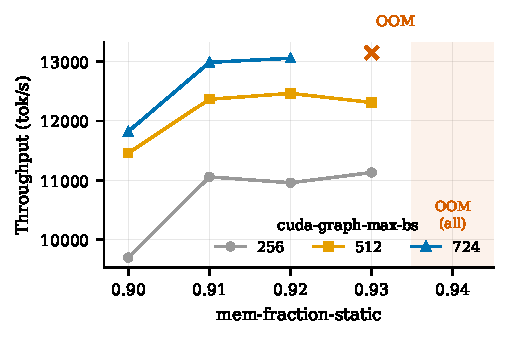
\includegraphics[width=\columnwidth]{figures/memfrac.pdf}
\caption{Throughput versus \texttt{mem-fraction-static} at three \texttt{cuda-graph-max-bs} settings (System~B, two nodes, TP=16, containerized). Larger KV-cache reservations and wider CUDA-graph coverage help---until allocation fails. The 724 series OOMs at 0.93, and every setting OOMs at 0.94.}
\label{fig:memfrac}
\end{figure}

With the stack fixed, the dominant remaining lever is keeping the GPUs saturated. Offline throughput is maximized when the continuous-batching scheduler~\cite{yu2022orca,kwon2023vllm} can pack as many concurrent requests as possible into the KV-cache: larger effective batches raise arithmetic intensity and amortize kernel-launch and scheduling overhead~\cite{pope2023efficiently}.

Figure~\ref{fig:memfrac} sweeps the two knobs jointly on System~B (two-node TP=16, containerized). The knobs compete for the same memory: \texttt{mem-fraction-static} reserves memory for weights and KV-cache, while capturing CUDA graphs for larger decode batches consumes part of the remainder. Raising \texttt{cuda-graph-max-bs} from 256 to 724---keeping large decode batches on the fast graph-replay path instead of eager launches---is worth 1{,}500--2{,}000 tok/s at every memory fraction; raising \texttt{mem-fraction-static} from 0.90 to 0.92 adds a further $\sim$1{,}200 tok/s at the widest graph coverage, peaking at 13{,}059 tok/s. Then the configuration space ends abruptly: 0.93 with graph capture to 724 fails with CUDA out-of-memory, as does 0.94 at every setting. Peak performance lives in a narrow window directly adjacent to the OOM cliff.

Workload volume matters symmetrically: in later single-node experiments, halving the prompt count from 2{,}000 to 1{,}000 dropped throughput disproportionately, from $\sim$17{,}000 to $\sim$10{,}000 tok/s, because the tail of the run drains the batch and leaves compute idle. Throughput benchmarks of batch-oriented LLM serving are, to first order, measurements of \emph{sustained batch occupancy}.

\subsection{Hybrid parallelism: TP4$\cdot$DP4$\cdot$PP2 with DP-attention}
\label{sec:hybrid}
\begin{table}
\caption{Parallelism layouts on a single System-B node (8$\times$H200, containerized; both runs shown where repeated).}
\label{tab:hybrid}
\small
\begin{tabular}{@{}llr@{}}
\toprule
\textbf{Layout} & \textbf{DP-attention} & \textbf{tok/s} \\
\midrule
TP=8 & off & 12{,}449 \\
TP=4, PP=2 & off & 12{,}537 / 11{,}436 \\
TP=2$\cdot$DP=2$\cdot$PP=4 & on & 16{,}499 / 15{,}229 \\
\textbf{TP=4$\cdot$DP=4$\cdot$PP=2} & \textbf{on} & \textbf{17{,}308 / 17{,}218} \\
\bottomrule
\end{tabular}
\end{table}

Having established single-node superiority, we searched the intra-node parallelism space (Table~\ref{tab:hybrid}). The winning layout composes all three axes: pipeline parallelism splits the model into two stages of four GPUs; within each stage, tensor parallelism spans four GPUs; and data-parallel attention runs four attention replicas per stage, each owning a disjoint shard of the running requests.

The layout works because each axis is matched to the resource it stresses. PP=2 halves the per-GPU weight footprint and confines TP's per-layer all-reduces to four-GPU NVLink islands. DP-attention addresses MLA's single-latent-head structure directly: under pure TP the compressed KV-cache is replicated on all ranks of the TP group, so a TP=4 group stores every cached token four times; with DP=4 attention each request's cache lives on exactly one rank. The recovered memory feeds directly into the batch capacity that Section~\ref{sec:batch} showed governs throughput, and enabling DP-attention additionally activates SGLang's shared-expert optimizations for DeepSeek models~\cite{sglangv04blog}. The effect is large: at fixed TP=4$\cdot$PP=2, turning DP-attention on is worth +38\% (12{,}537 $\rightarrow$ 17{,}308 tok/s). Composing parallelism naively, by contrast, is not enough---TP=2$\cdot$DP=2$\cdot$PP=4 trails the winner by $\sim$1{,}500 tok/s, with deeper pipelining providing too little intra-stage compute to hide stage handoffs.

The final configuration also enabled SGLang's \texttt{torch.compile} integration; in isolation this flag produced no measurable difference in our earlier tests, consistent with SGLang's own kernels already dominating the profile.

\subsection{NCCL tuning: an instructive null result}
\label{sec:nccl}
\begin{figure}
\centering
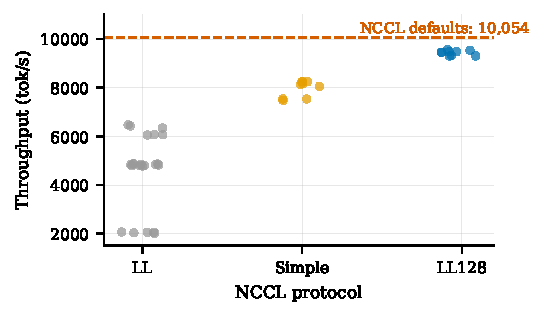
\includegraphics[width=\columnwidth]{figures/nccl.pdf}
\caption{Forty manually tuned NCCL configurations (System~B, two nodes, TP=16), grouped by protocol. No manual configuration reaches the autotuned default (dashed line, 10{,}054 tok/s).}
\label{fig:nccl}
\end{figure}

Before abandoning multi-node scaling we asked whether the inter-node penalty was merely a communication-library misconfiguration. We swept NCCL's~\cite{nccl} tuning surface on the two-node TP=16 configuration: protocol (\texttt{LL}, \texttt{LL128}, \texttt{Simple}), thread count (64--256), minimum channels (4--16), CUDA device connections, PCI relaxed ordering, socket threads, and GPU-Direct RDMA level---40 configurations in total.

Figure~\ref{fig:nccl} shows the outcome: every manual configuration (2{,}019--9{,}561 tok/s) lost to NCCL's defaults (10{,}054 tok/s). The sweep is still informative about mechanism. Protocol dominates: \texttt{LL128} ($\le$9{,}561) $>$ \texttt{Simple} ($\le$8{,}251) $>$ \texttt{LL} ($\le$6{,}475). Disabling GPU-Direct RDMA is catastrophic, cutting throughput 2.4$\times$ (e.g., 4{,}866 $\rightarrow$ 2{,}035 tok/s at otherwise identical settings); within the GDR-enabled regime, relaxing the locality threshold monotonically helps (9{,}452 tok/s when GDR is never used, rising through PCI, root-complex, and NUMA locality levels to 9{,}761 when always used). Modern NCCL probes topology and selects algorithms dynamically; a static configuration cannot beat it, and the two-node penalty of Section~\ref{sec:scaling} is therefore attributable to the fabric itself rather than to library settings.

As a final micro-tuning pass we swept \texttt{NCCL\_NET\_GDR\_LEVEL} on the best single-node configuration, observing 17{,}255, 17{,}352, and 17{,}417 tok/s at levels 2, 3, and 5. The spread ($\sim$1\%) is within plausible run-to-run variance; we report the best observed run, obtained at level 5, as our final figure.

\subsection{End-to-end result and per-GPU efficiency}
\label{sec:final}
\begin{figure}
\centering
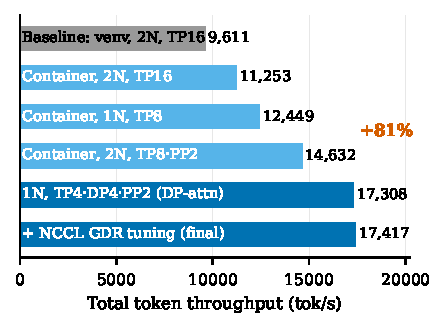
\includegraphics[width=\columnwidth]{figures/ladder.pdf}
\caption{The optimization ladder on System~B. Light bars are intermediate steps; dark bars are the final hybrid configuration. The final single-node configuration improves 81\% over the two-node baseline while using half the GPUs.}
\label{fig:ladder}
\end{figure}

\begin{figure}
\centering
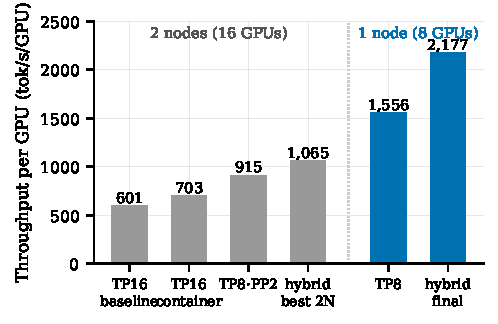
\includegraphics[width=\columnwidth]{figures/pergpu.pdf}
\caption{Per-GPU throughput. The tuned single-node configuration (right) more than doubles the per-GPU efficiency of the best two-node configuration and reaches 3.6$\times$ the baseline.}
\label{fig:pergpu}
\end{figure}

Figure~\ref{fig:ladder} assembles the ladder: from the untuned two-node baseline (venv, TP=16; 9{,}611 tok/s), through containerization, the retreat to a single node, pipeline-based node crossing, and finally the hybrid TP4$\cdot$DP4$\cdot$PP2 layout with DP-attention, landing at 17{,}417 tok/s: \textbf{+81\%} over baseline on half the hardware. The final run processed 2{,}000 requests (626{,}729 input + 388{,}685 generated tokens) in 58.3\,s---comfortably inside the 420\,s budget---at 34.3 requests/s.

For completeness we also ran the winning hybrid layout across both nodes (16 GPUs): it reached 17{,}032 tok/s, \emph{still below the single node}. Figure~\ref{fig:pergpu} recasts the comparison in per-GPU terms: 2{,}177 tok/s per GPU on one node versus 1{,}065 on two---a 2.05$\times$ efficiency gap, and 3.6$\times$ the baseline's 601. Under any resource-accounting model in which GPUs have a price, the single-node deployment is strictly dominant for this workload: it is faster in absolute terms and frees eight GPUs to serve a second replica.

\section{Discussion}
\label{sec:discussion}
\paragraph{Guidance for practitioners.}
Our measurements compress into five rules. (1)~\emph{Pin and modernize the stack}: CUDA toolkit alignment and a maintainer-built container were worth +35\% and +12\% respectively, at zero algorithmic cost. (2)~\emph{Scale vertically first}: exhaust the NVLink domain before touching the inter-node fabric; a monolithic MoE model of this scale is served best from the largest single NVLink island that fits it. (3)~\emph{If you must cross nodes, cross with pipeline parallelism}, which moves per-microbatch activations rather than per-layer collectives. (4)~\emph{Feed the batch scheduler}: reserve as much KV-cache memory as the OOM cliff allows, minus an operational safety margin---the peak sits directly against the cliff, and a production configuration tuned to the edge is brittle against long requests. (5)~\emph{Trust NCCL's defaults}; spend the tuning budget on parallelism layout instead.

\paragraph{Scaling out by replication.}
The natural way to use the second node is not to couple it into the model but to run a second, independently tuned replica behind a request router. SGLang's offline benchmark cannot express this infrastructure-level data parallelism, so as a preliminary check we deployed two single-node servers behind the SGLang router~\cite{sglangrouter} in online-serving mode, observing 8{,}438 tok/s. The number is not comparable to our offline figures---it traverses the HTTP serving path with per-request scheduling rather than a pre-materialized offline batch---and router-based scaling of tuned workers remains the deployment architecture we would take to production, with proper online benchmarking (goodput under latency SLOs) as future work.

\paragraph{Threats to validity.}
Most configuration points are single runs, a limitation imposed by the shared-cluster time budget; the repeated points suggest $\sim$1\% variance on tuned configurations, so we avoid interpreting sub-2\% deltas. The venv-versus-container comparison conflates a minor framework version change with the runtime. Dummy weights preserve compute and memory but preclude output-quality checks. Results are for one model family, one serving framework, and offline throughput; latency-bounded online serving may prefer different layouts. Cross-system numbers (H100 versus H200) are never compared directly, and per-system conclusions (stack sensitivity on System~A; scaling and parallelism on System~B) should be read within their system.

\section{Related Work}
Continuous batching and paged KV-cache management were introduced by Orca~\cite{yu2022orca} and vLLM~\cite{kwon2023vllm}; SGLang~\cite{zheng2024sglang} adds RadixAttention prefix reuse and the DeepSeek-specific optimizations central to this paper~\cite{sglangv04blog}. Tensor and pipeline parallelism originate in the training literature~\cite{shoeybi2019megatron,huang2019gpipe,narayanan2021efficient}; Pope et al.~\cite{pope2023efficiently} analyze their trade-offs for dense-model inference on TPU pods, reaching a conclusion consonant with ours---partitioning must follow the interconnect hierarchy. Our study differs in targeting a production MoE reasoning model on commodity-cloud-class H100/H200 nodes, in quantifying the software-stack terms (toolkit, container) that deployment guides usually assume away, and in reporting the negative space (NCCL manual tuning, cross-node TP) that practitioners otherwise rediscover at their own expense.

\section{Conclusion}
We presented a systematic, log-verified benchmarking campaign of DeepSeek-R1 offline inference with SGLang on two production GPU systems. Intelligent configuration---toolkit alignment, containerization, KV-cache-aware batching, and a hybrid TP4$\cdot$DP4$\cdot$PP2 layout exploiting DP-attention---delivered 17{,}417 tok/s on a single 8$\times$H200 node, an 81\% improvement over the two-node baseline and a 2.05$\times$ per-GPU efficiency advantage over the best 16-GPU configuration. The broader lesson for benchmarking in the data center is that for tightly coupled LLM inference, the unit of scaling is the NVLink domain: configuration quality within it, and replication across it, beat raw GPU count every time we measured the alternative.

\begin{acks}
We thank the National Supercomputing Centre (NSCC) Singapore for access to ASPIRE-2A+, the operators of the H200 system for cluster access, the HPC-AI Advisory Council for organizing the 2025 APAC HPC-AI Competition, and our Monash DeepNeuron teammates for the HPC track of the competition.
\end{acks}

\bibliographystyle{ACM-Reference-Format}
\bibliography{refs}

\end{document}
